\documentclass[10pt]{beamer}
\usepackage[ngerman]{babel}

\usetheme[background=light,everytitleformat=regular,inner/sectionpage=progressbar,block=fill]{m}

\usepackage[numbers,round]{natbib}
\usepackage{amsmath}
\usepackage{mathtools}
\usepackage{amssymb}
\usepackage{booktabs}
\usepackage{multicol}
\usepackage[scale=2]{ccicons}

\title{Fourieranalyse}
\subtitle{Hintergrund und Anwendungen von Frequenzanalysen}
\date{\today}
\author{Adrian Schrader}
\institute{Physik 4h, Herr Kuhn}

\begin{document}

\section{Motivation}

\frame{
  \begin{figure}
    \centering
    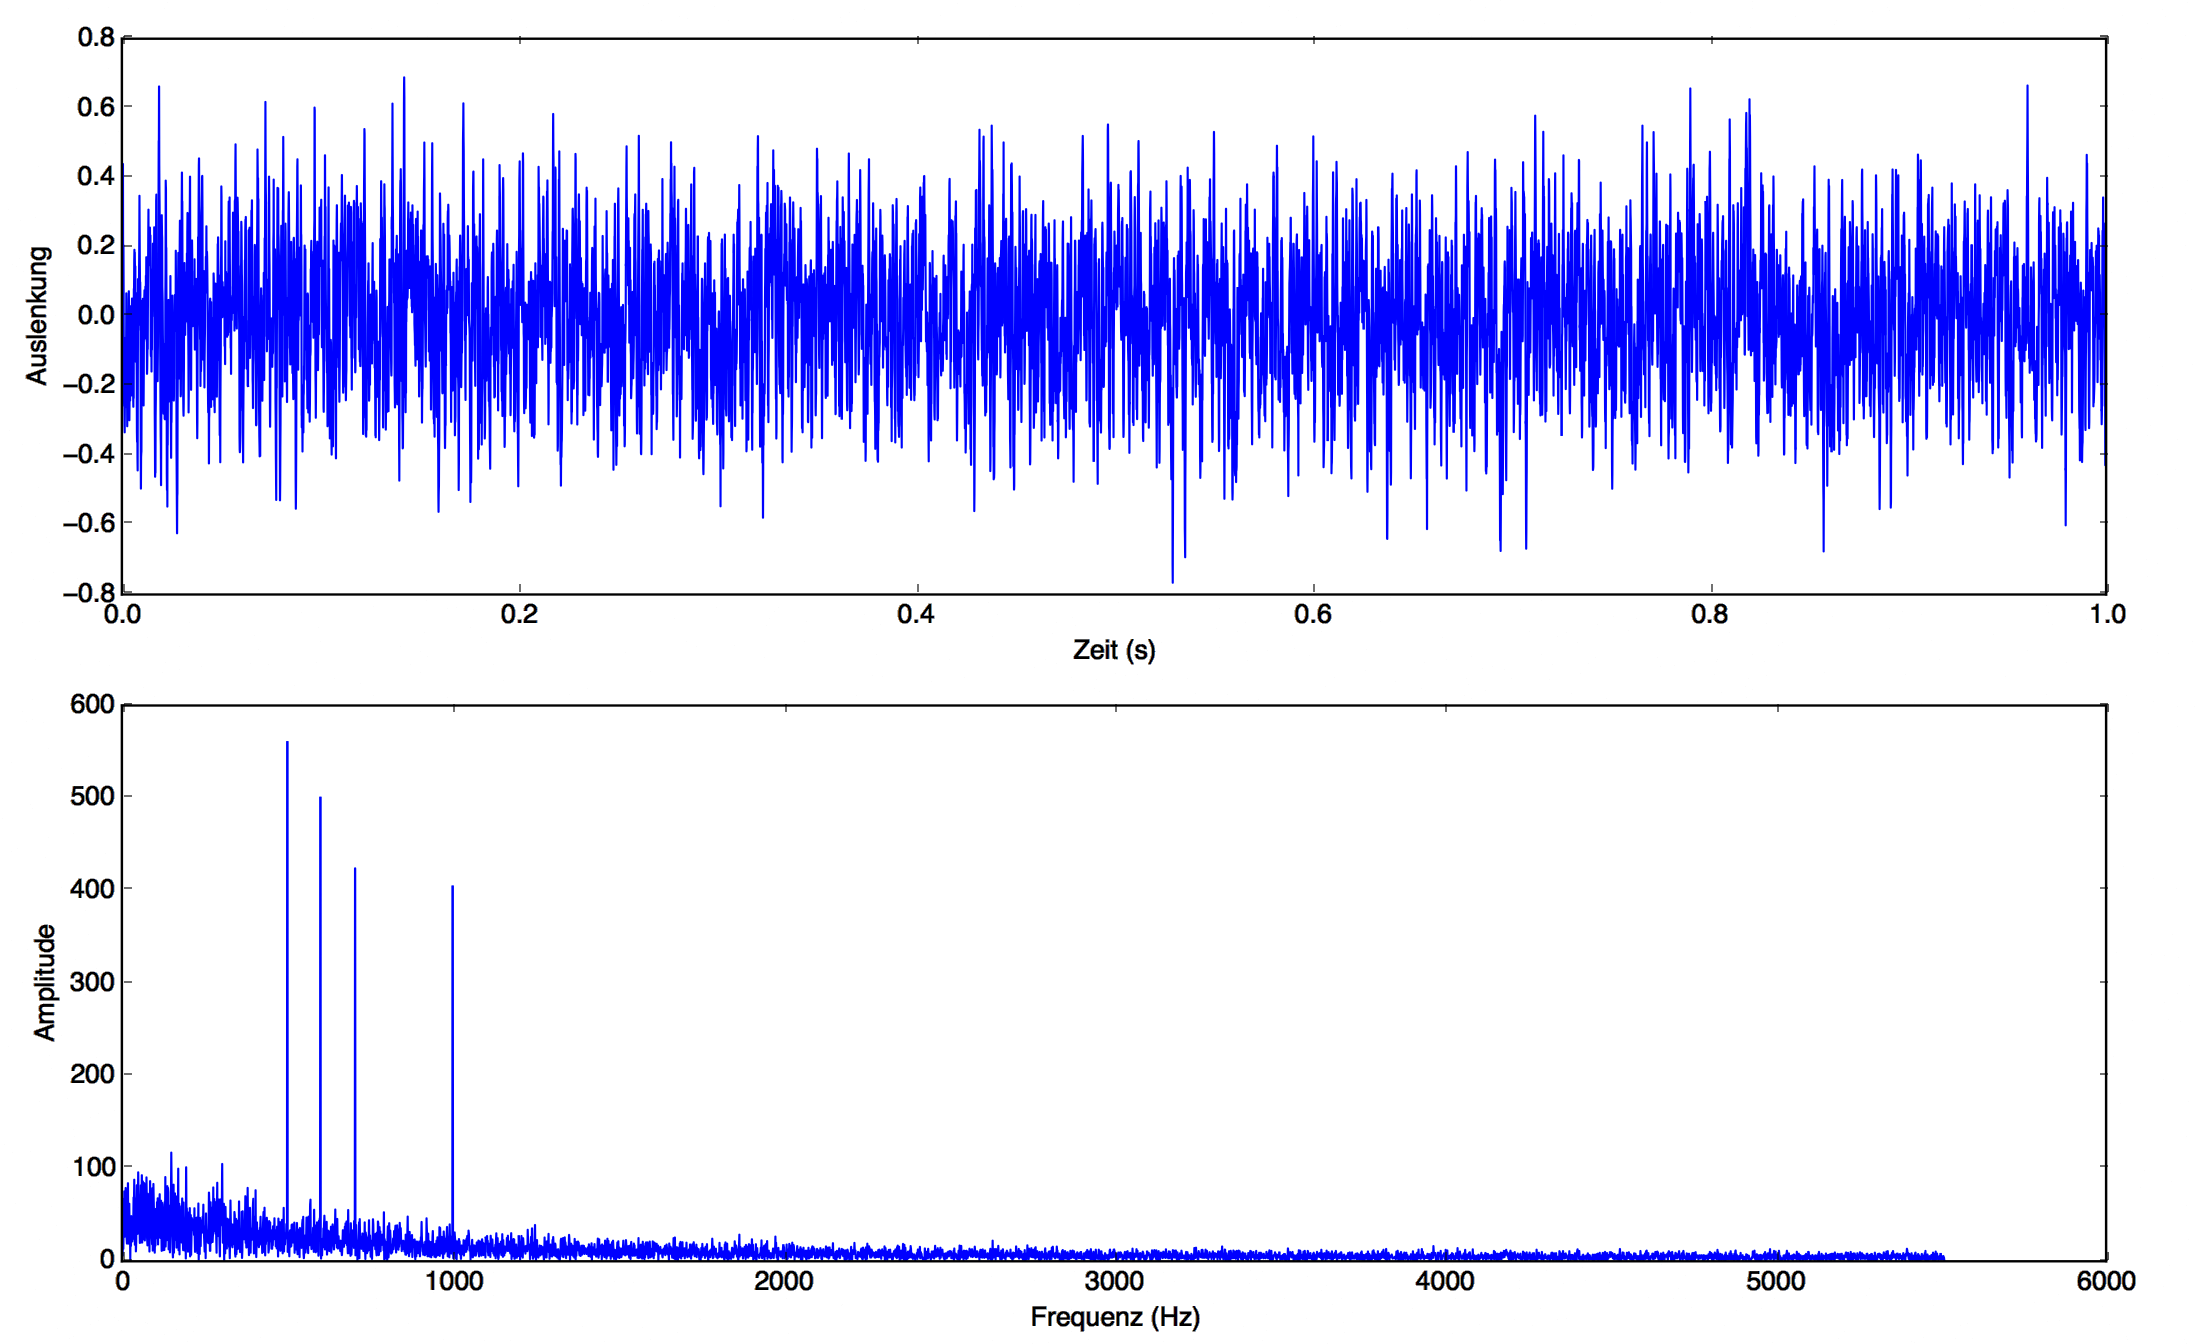
\includegraphics[width=\linewidth]{img/introduction}
    \label{img:introduction}
  \end{figure}
}


\maketitle

\begin{frame}
  \frametitle{Inhaltsübersicht}
  \setbeamertemplate{section in toc}[sections numbered]
  \tableofcontents
\end{frame}

% ----  CONTENT  ----
\section{Einführung und Herleitung}

\begin{frame}
  \frametitle{Aufgabenstellung}

  \begin{figure}
    \centering
    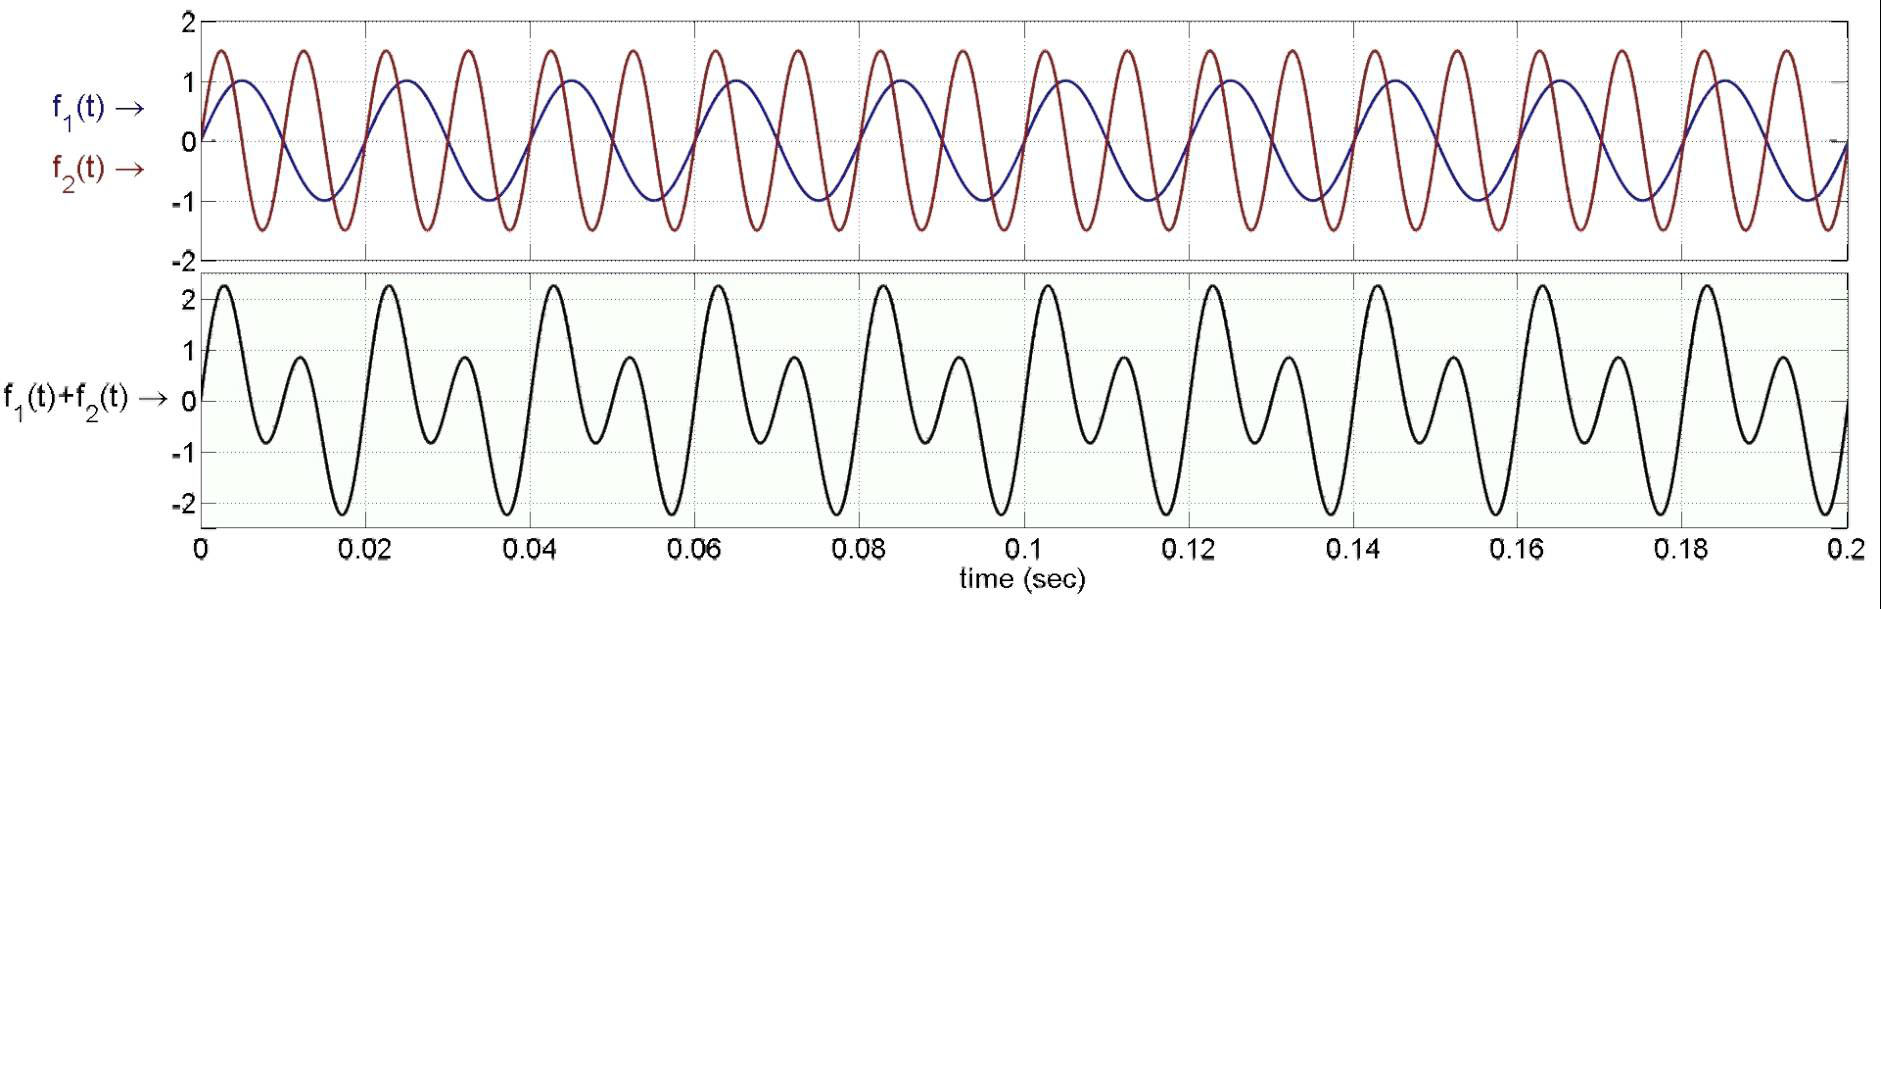
\includegraphics[width=\linewidth]{img/intro_transform1}
    \caption{Beispiel einer Fouriertransformation (https://i.ytimg.com/vi/-GYB7khbIA0/maxresdefault.jpg, 08.11.15)}
  \end{figure}
\end{frame}

\begin{frame}
  \frametitle{Aufgabenstellung}

  \begin{figure}
    \centering
    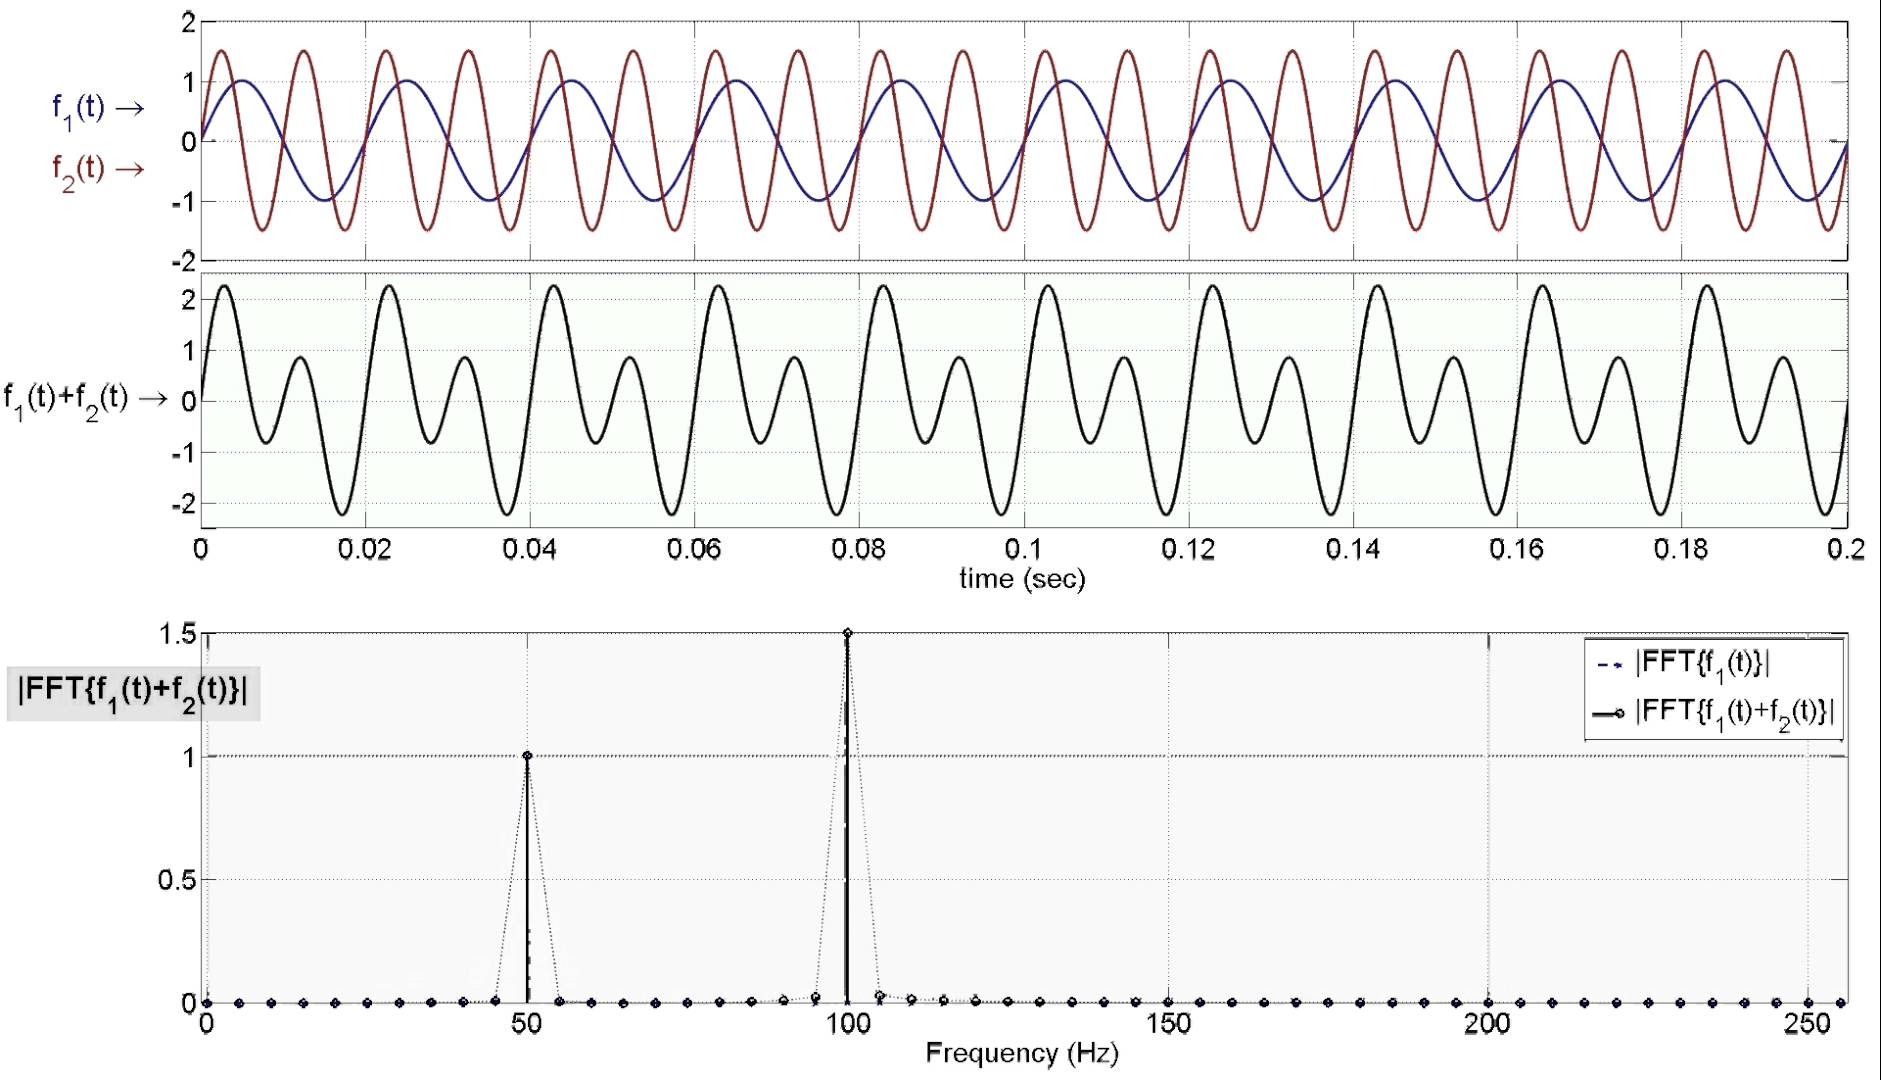
\includegraphics[width=\linewidth]{img/intro_transform2}
    \caption{Beispiel einer Fouriertransformation (https://i.ytimg.com/vi/-GYB7khbIA0/maxresdefault.jpg, 08.11.15)}
  \end{figure}
\end{frame}

\begin{frame}
  \frametitle{Grund- und Oberschwingungen}

  \begin{align*}
    \begin{split}
      f(t) = \frac{a_0}{2} &+ a_1 \cdot cos(t) + a_2 \cdot cos(2 t) + a_3 \cdot cos(3 t) + ... \\ &+ b_1 \cdot sin(t) + b_2 \cdot sin(2 t) +  b_3 \cdot sin(3 t) + ... \\
    \end{split}
  \end{align*}

  \begin{align*}
    f(t) &= \alpha_0 + \alpha_1 \cdot e^{i \cdot t} + \alpha_2 \cdot e^{i \cdot ( 2 t)} + \alpha_3 \cdot e^{i \cdot (3 t)} + ... \\
         &= \sum_{n = 0}^{\infty} \alpha_n \cdot e^{i\cdot  n\cdot  t}
  \end{align*}
  \begin{align*}
    e^{i \cdot n \cdot t} = cos(n \cdot t) + i \cdot sin(n \cdot t) && i^2 = -1
  \end{align*}
\end{frame}

\begin{frame}
  \frametitle{Mathematische Herleitung}

  \begin{align*}
    e^{i \cdot n \cdot t} = cos(n \cdot t) + i \cdot sin(n \cdot t) && \{ n \not= m \, \text{  und  } \, n, m \in \mathbb{Z} \}
  \end{align*}

  \begin{align*}
    &\int_{-\pi}^{\pi} e^{i \cdot n \cdot t} \, dt &&  &&= 0 \\
    &\int_{-\pi}^{\pi} e^{i \cdot n \cdot t} \cdot e^{-i \cdot m \cdot t} \, dt &&= \int_{-\pi}^{\pi} e^{i \cdot (n - m) \cdot t} \, dt &&= 0 \\
    &\int_{-\pi}^{\pi} e^{i \cdot n \cdot t} \cdot e^{-i \cdot n \cdot t} \, dt &&= \int_{-\pi}^{\pi} e^{0} \, dt &&= 2 \pi
  \end{align*}


\end{frame}

\begin{frame}
  \frametitle{Mathematische Herleitung}

  \begin{align*}
f(t) &= \alpha_0 + \alpha_1 \cdot e^{i \cdot t} + \alpha_2 \cdot e^{i \cdot ( 2 t)} + \alpha_3 \cdot e^{i \cdot (3 t)} + ...
  \end{align*}

  \only<1>{
  \begin{align*}
    \int_{-\pi}^{\pi} f(t) \cdot e^{-i \cdot (2 t)} \, dt &= \int_{-\pi}^{\pi} \alpha_0 \cdot e^{-i \cdot (2 t)} \, dt \\
    &+ \int_{-\pi}^{\pi} \alpha_1 \cdot e^{i \cdot t} \cdot e^{-i \cdot (2 t)} \, dt \\
    &+ \int_{-\pi}^{\pi} \alpha_2 \cdot e^{i \cdot (2 t)} \cdot e^{-i \cdot (2 t)}\, dt \\
    &+ \int_{-\pi}^{\pi} \alpha_3 \cdot e^{i \cdot (3 t)} \cdot e^{-i \cdot (2 t)}\, dt \\
    &+ ...
  \end{align*}
  }
\end{frame}

\begin{frame}
  \frametitle{Fourier-Transformaton}

  \begin{align*}
    \int_{-\pi}^{\pi} f(t) \cdot e^{-i \cdot (2 t)} \, dt &= 0 + 0 + 2 \pi \cdot \alpha_2 + 0 + 0 ... \\
    &= 2 \pi \cdot \alpha_2
  \end{align*}

  \only<2>{
  \begin{align*}
    \mathcal{F}(f)(\omega) = \hat{f}(\omega) = \frac{1}{2\pi} \int_{-\pi}^{\pi} f(t) \cdot e^{-i \cdot n \cdot t} \, dt \\
  \end{align*}
  }
\end{frame}

\section{Diagramme und Darstellungen}

\begin{frame}
  \frametitle{FFT und Frequenzspektren}
  \begin{figure}
    \centering
    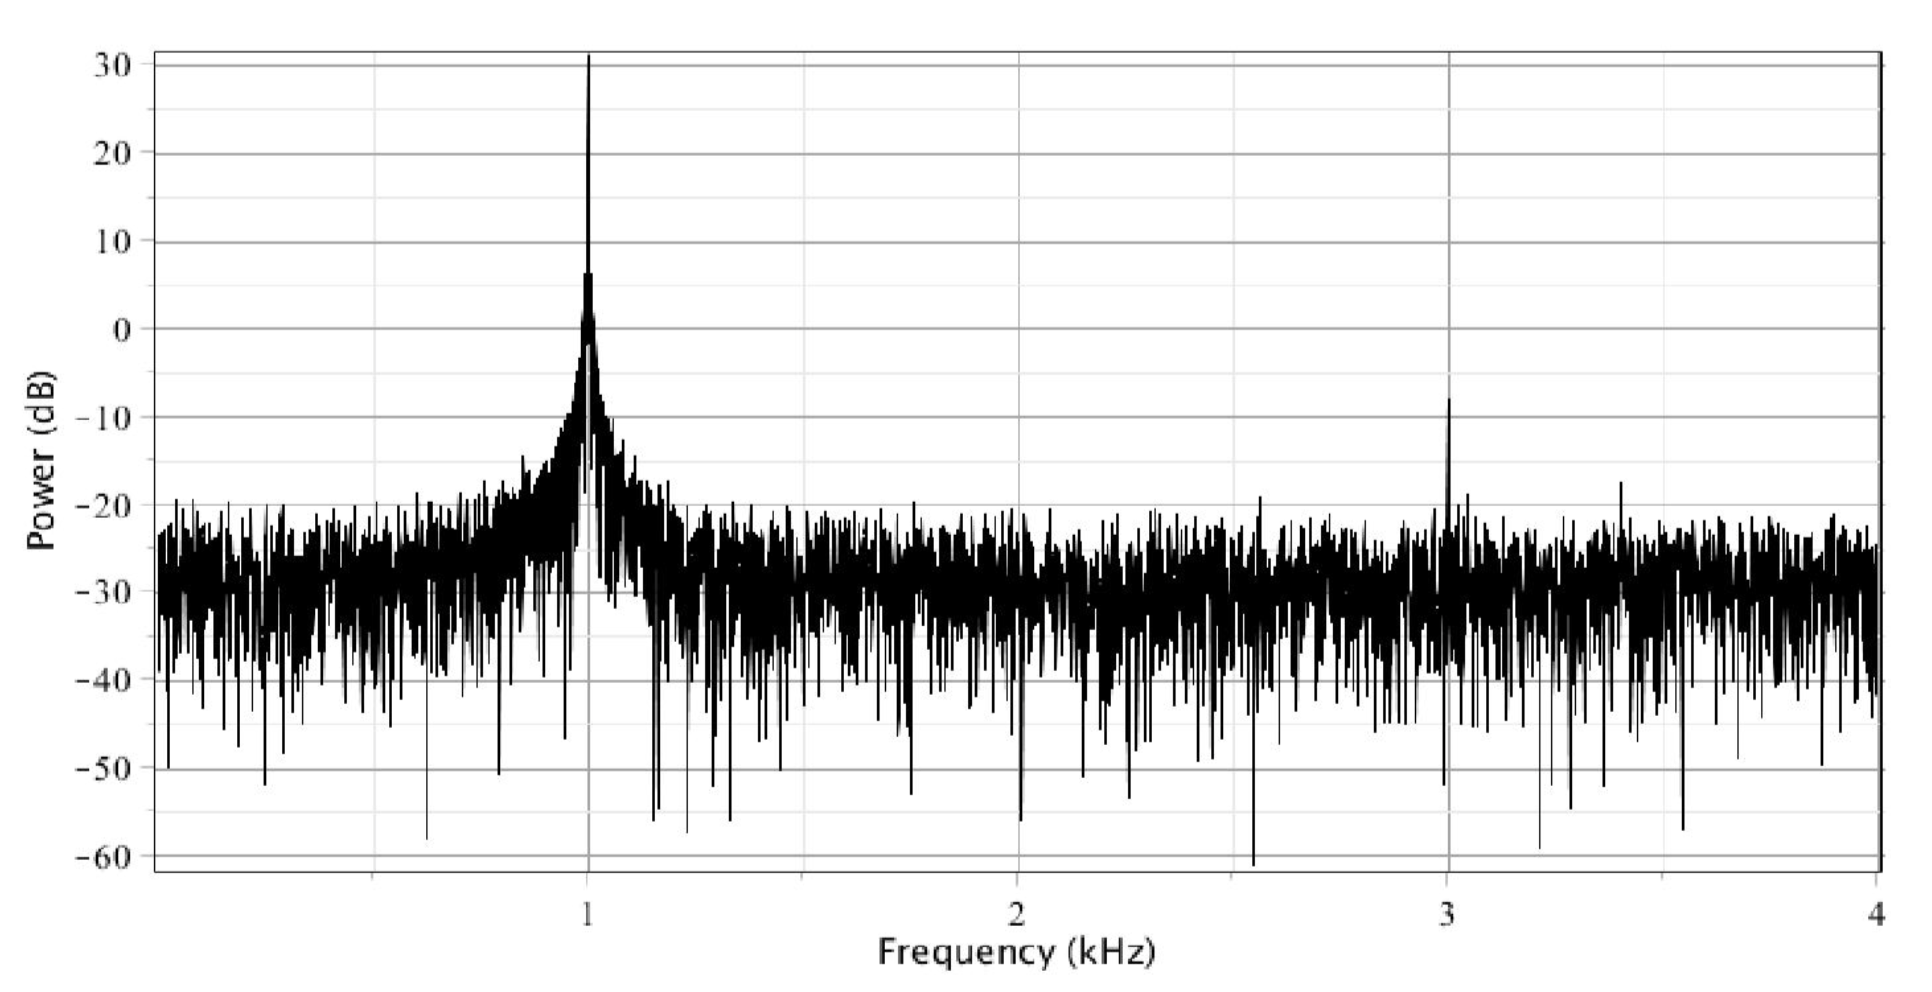
\includegraphics[width=\linewidth]{img/1khz_power}
    \caption{\url{ http://www.maplesoft.com/products/maple/features/Signal_Processing.aspx},  21.11.15}
  \end{figure}
\end{frame}

\begin{frame}
  \frametitle{Spektrogramme}
  \begin{figure}
    \centering
    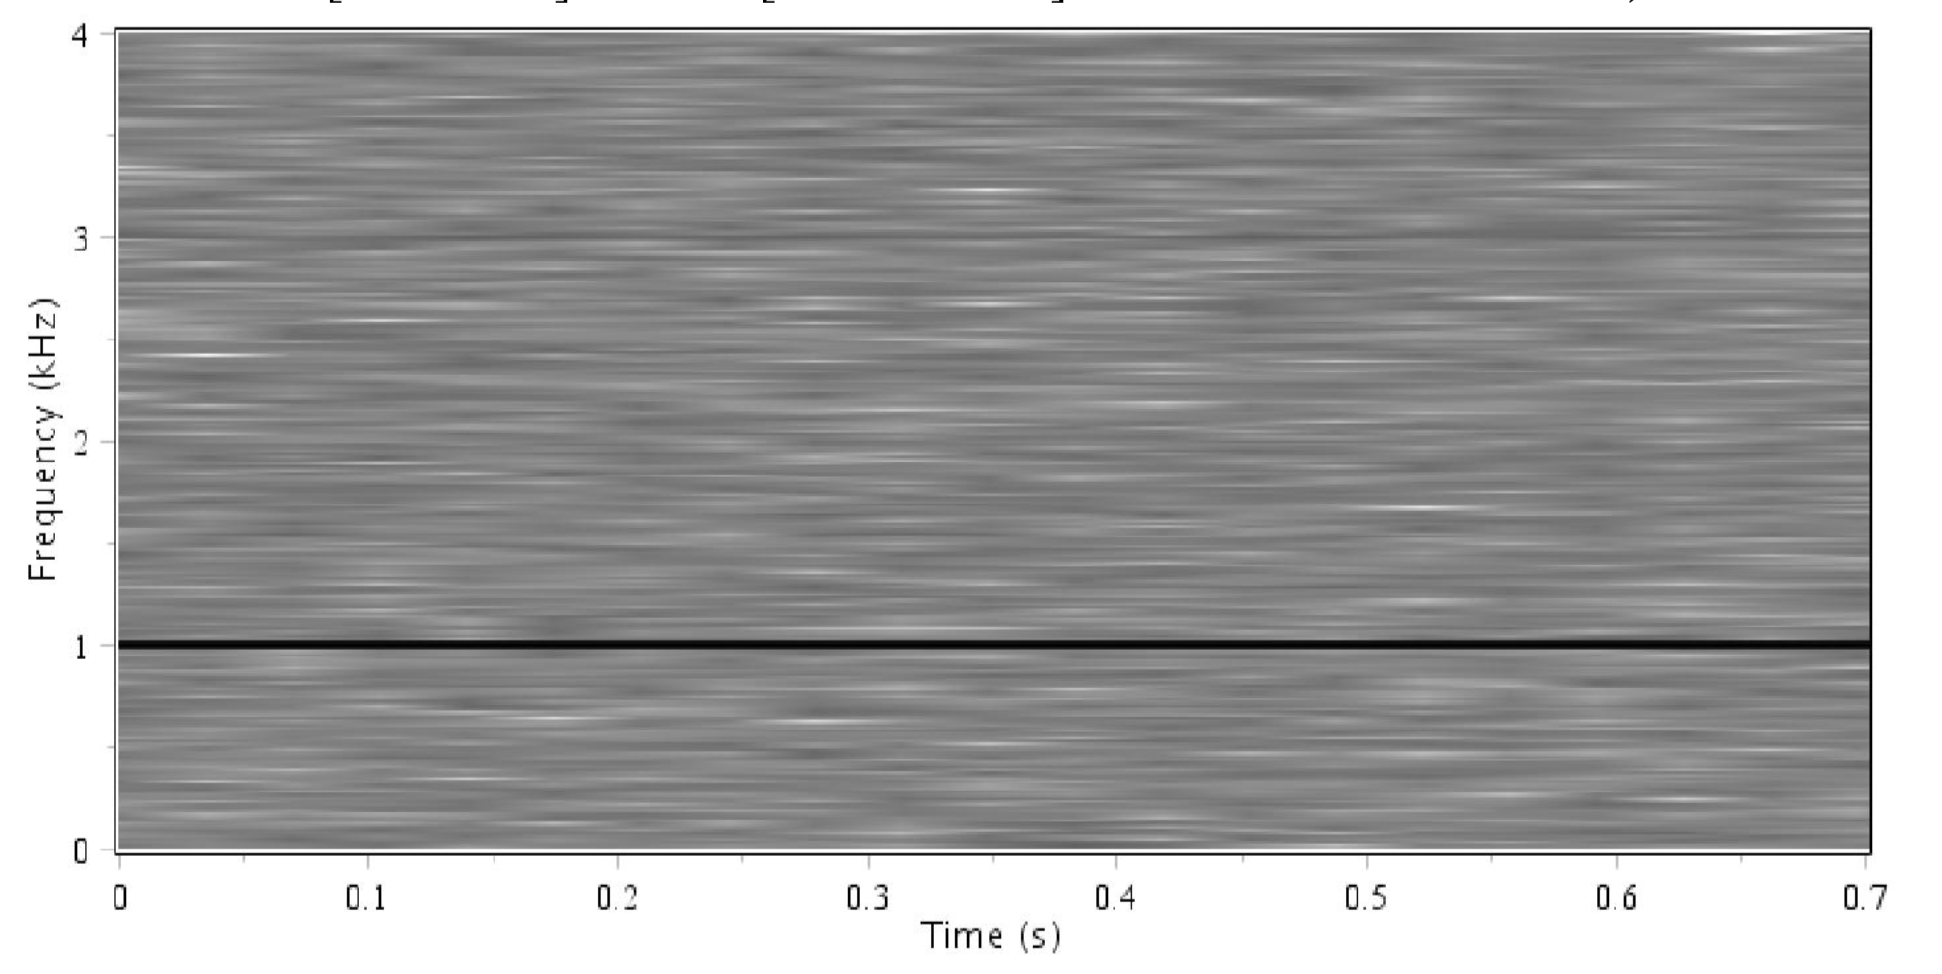
\includegraphics[width=\linewidth]{img/1khz}
    \caption{\url{ http://www.maplesoft.com/products/maple/features/Signal_Processing.aspx}, 21.11.15}
  \end{figure}
\end{frame}

\section{Anwendungen und Beispiele}

\subsection{Klangwiedergange einer Geige}

\begin{frame}
  \frametitle{Klangcharakteristika einer Geige}
  \begin{figure}
    \centering
    \only<1>{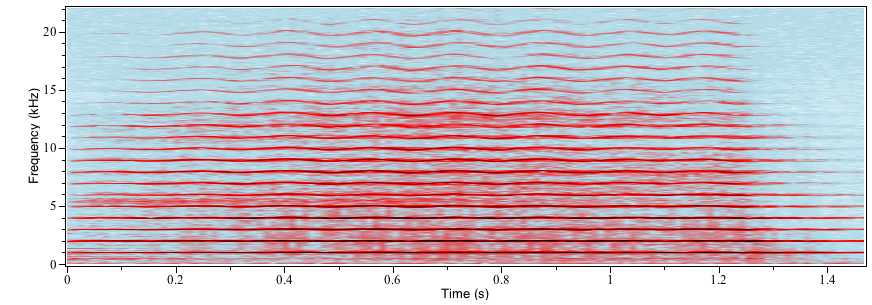
\includegraphics[width=\linewidth]{img/violin}}
    \only<2>{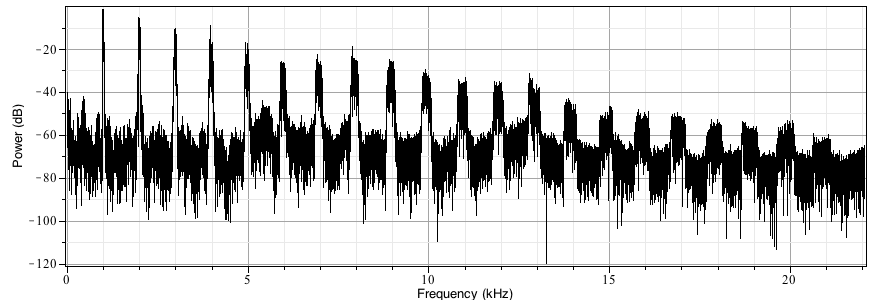
\includegraphics[width=\linewidth]{img/violin_power}}
    \label{img:violin}
  \end{figure}
\end{frame}

\subsection{Charakteristika von Sprache}

\begin{frame}
  \frametitle{Sprache}
    \begin{figure}
      \centering
      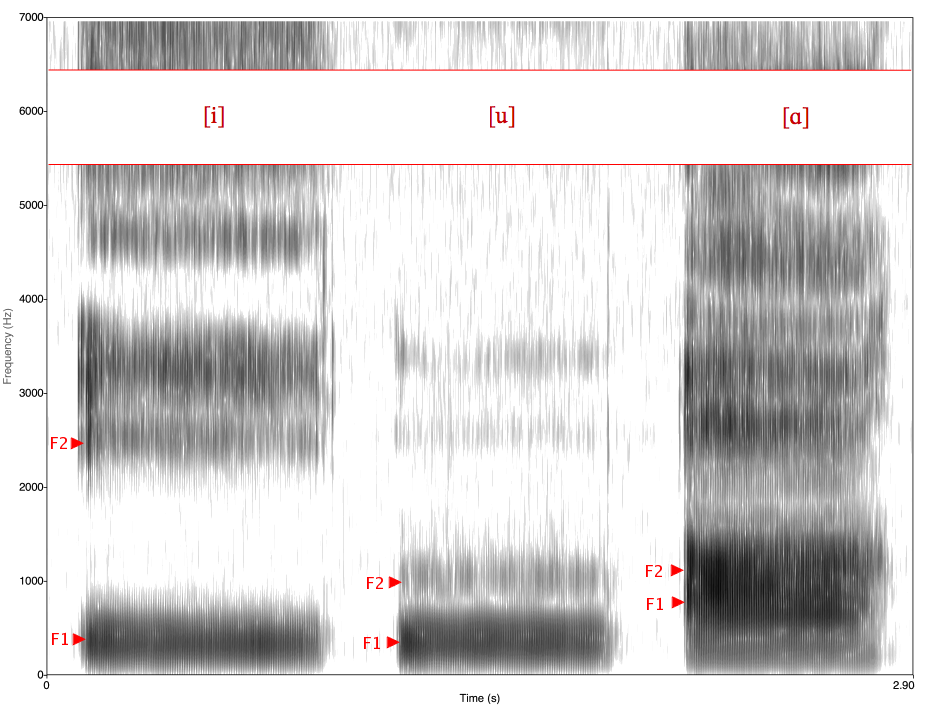
\includegraphics[width=0.8\linewidth]{img/iua}
      \label{img:vowls}
      \caption{\url{https://commons.wikimedia.org/wiki/File:Spectrogram_-iua-.png}, 02.12.15}
    \end{figure}
\end{frame}

\begin{frame}
  \frametitle{Sprache}
    \begin{figure}
      \centering
      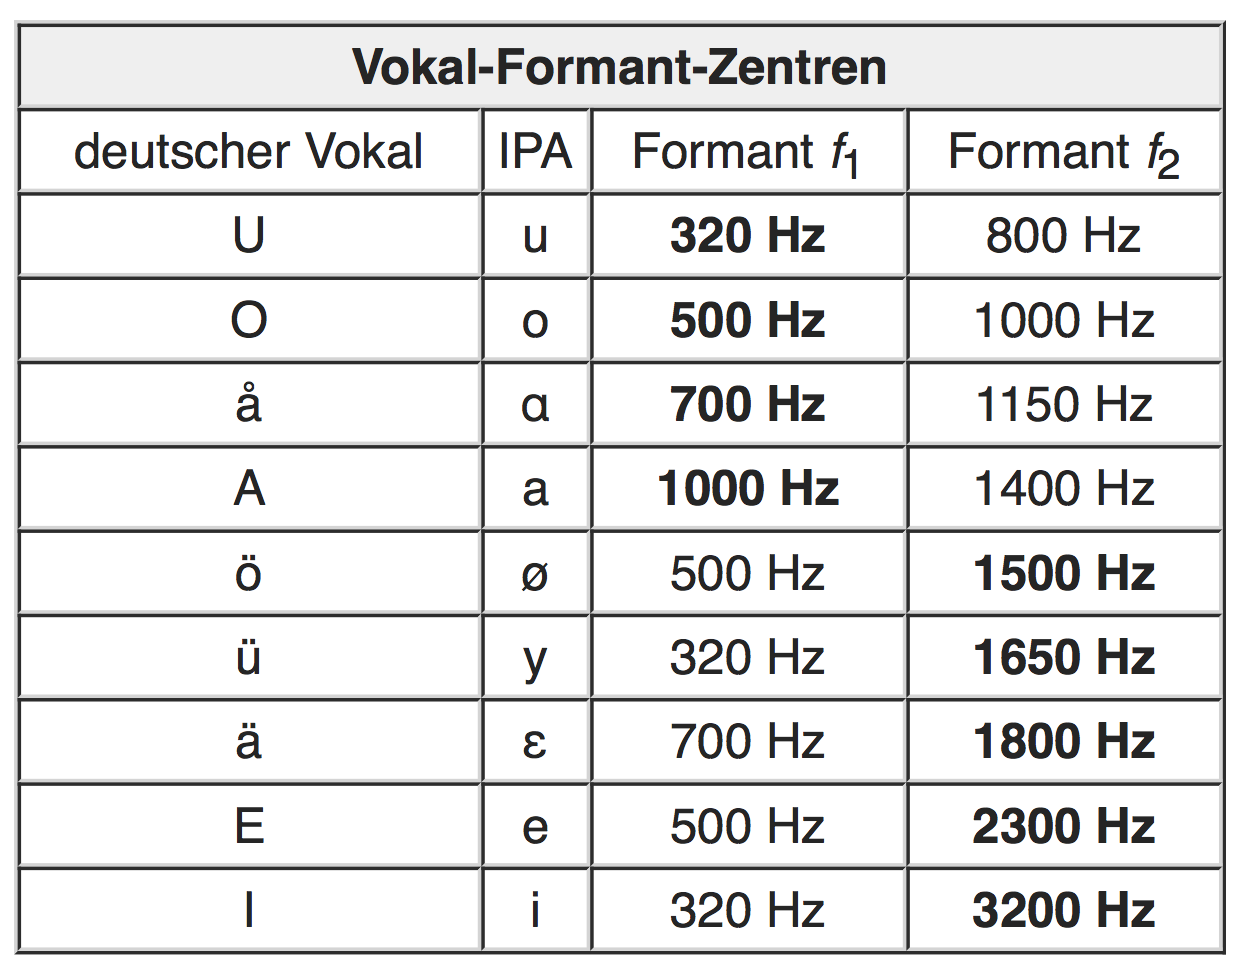
\includegraphics[width=0.8\linewidth]{img/formanten}
      \label{img:vowls}
    \end{figure}
\end{frame}


\plain{Fragen?}

\begin{frame}[allowframebreaks]

  \nocite{*}
  \bibliography{bib/bibliography}
  \bibliographystyle{abbrv}

\end{frame}

%\section*{Anhang: Vorbereitete Fragen}

\begin{frame}
  \only<1>{
  \begin{exampleblock}{Leitfrage}
    \begin{quotation}
      Die Art von Informationen, die ein Mensch mit einem Cochlea-Implantat beim Musikhören bekommt, ist so, als würde jemand am Klavier nicht mit einzelnen Fingern eine Melodie spielen, sondern mit seinen kompletten Unterarmen. Die einzelnen Elektroden der Cochlea-Implantate decken jeweils ein so breites Frequenzspektrum ab, dass sich Tonhöhen kaum unterscheiden lassen.
    \end{quotation}
  \end{exampleblock}}

  \only<2>{
  \begin{exampleblock}{Leitfrage}
    \begin{quotation}
      Die Art von Informationen, die ein Mensch mit einem \alert{Cochlea-Implantat} beim Musikhören bekommt, ist so, als würde jemand am Klavier nicht mit einzelnen Fingern eine Melodie spielen, sondern mit seinen kompletten Unterarmen. Die einzelnen Elektroden der Cochlea-Implantate decken jeweils ein so \alert{breites Frequenzspektrum} ab, dass sich Tonhöhen kaum unterscheiden lassen.
    \end{quotation}
  \end{exampleblock}}

\end{frame}

\subsection{Einstieg}
\begin{frame}
  \begin{figure}
    \centering
    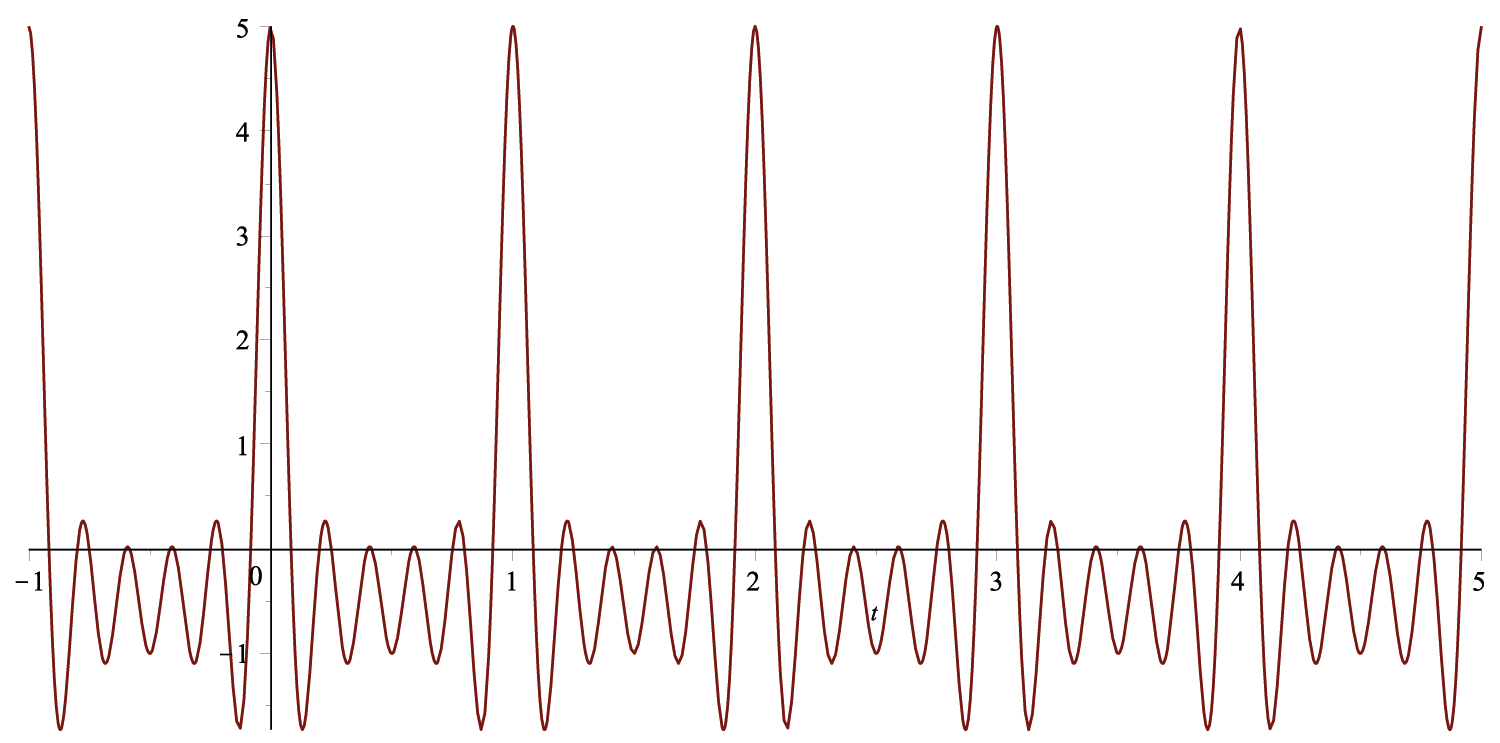
\includegraphics[width=\linewidth]{img/intro_harmonics}
    \caption{Auslenkungs-Zeit-Diagramm von Grund- und Oberschwingungen}
    \label{img:harmonics}
  \end{figure}
\end{frame}

\begin{frame}
  \begin{figure}
    \centering
    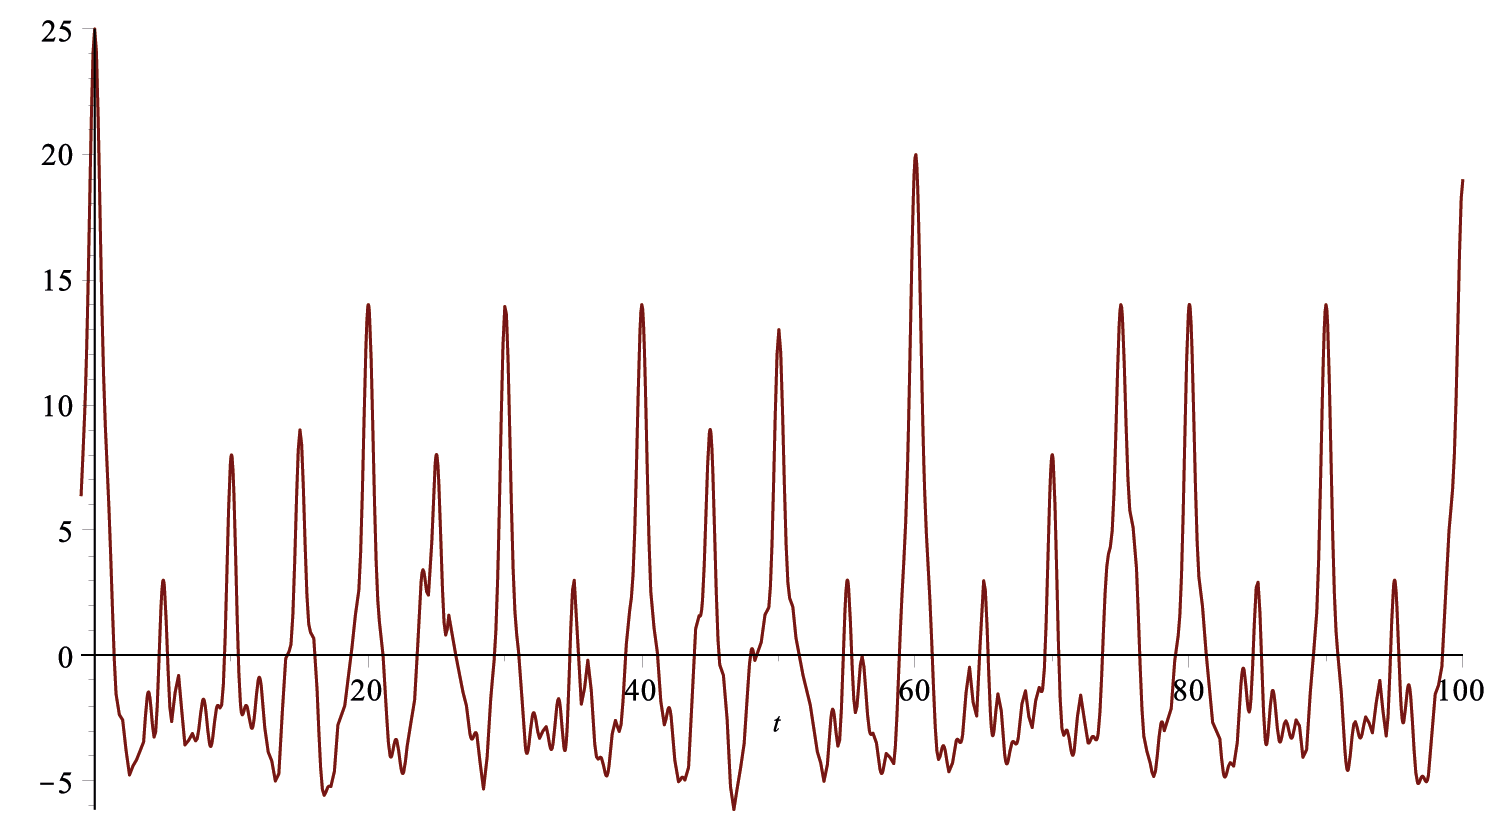
\includegraphics[width=\linewidth]{img/intro_interference}
    \caption{Auslenkungs-Zeit-Diagramm von verschiedenen Grund- und Oberschwingungen}
    \label{img:interference}
  \end{figure}
\end{frame}

\subsection{Mathematische Herleitung}
\begin{frame}
  \frametitle{Hilberträume}

  \begin{itemize}
    \item Vektorraum wird durch ein Skalarprodukt $ \langle f, g \rangle $ und Orthonormalbasen definiert
    \item \emph{Orthogonalität} bedeutet $\langle f, g \rangle = 0$
  \end{itemize}

  \begin{align*}
    \langle f, g \rangle = \int_{-\pi}^{\pi} f(x) \cdot g(x) \, dx
  \end{align*}
\end{frame}

\begin{frame}
  \frametitle{Orthonormalvektoren}

  \begin{align*}
    &\int_{-\pi}^{\pi} sin(k x) \, dx &&= 0 && \Rightarrow && sin(k x) \perp 1 \\
    &\int_{-\pi}^{\pi} cos(k x) \, dx &&= 0 && \Rightarrow && cos(k x) \perp 1 \\
    &\int_{-\pi}^{\pi} sin(k x)\cdot cos(m x) \, dx &&= 0 && \Rightarrow && sin(k x) \perp cos(m x) \\
    &\int_{-\pi}^{\pi} sin(k x)\cdot sin(m x) \, dx &&= \pi \cdot \delta_{m n} && \Rightarrow && sin(k x) \perp sin(m x), k \neq m \\
    &\int_{-\pi}^{\pi} cos(k x)\cdot cos(m x) \, dx &&= \pi \cdot \delta_{m n} && \Rightarrow && cos(k x) \perp cos(m x), k \neq m \\
    &\int_{-\pi}^{\pi} 1 \, dx &&= 2 \pi && \Rightarrow && 1 \not\perp 1
  \end{align*}
\end{frame}

\begin{frame}
  \frametitle{Fourieranalyse}

  \begin{align*}
    f(t) = \frac{a_0}{2} &+ a_1 \cdot cos(  t) + a_2 \cdot cos(2   t) + ... + a_n \cdot cos(n   t) \\ &+ b_1 \cdot sin( t) + b_2 \cdot sin(2  t) + ... + b_n \cdot sin(n  t)
   \end{align*}
   \begin{align*}
     \int_{-\pi}^{\pi} f(t) \cdot cos(n t) \, dx = &\int_{-\pi}^{\pi} \frac{a_0}{2} \cdot cos(n t) \,dx \\
      &+ a_n \int_{-\pi}^{\pi} cos(n  t) \cdot cos(n t) \, dx \\
      &+ b_n \int_{-\pi}^{\pi} sin(n  t) \cdot cos(n t) \, dx\\
      &= \pi \cdot a_n
    \end{align*}
\end{frame}


\end{document}
